
\begin{frame}{Learning Movement Primitives for the Humanoid Robot HRP2}
  \framesubtitle{(EKUT, CNRS-LAAS)}
  %\vspace*{-0.8cm}  
  \begin{center}
    \scalebox{0.7}{\newcommand{\picturefontsize}{\LARGE}
\newcommand{\pictureLineWidth}{0.8mm}

% For every picture that defines or uses external nodes, you'll have to
% apply the 'remember picture' style. To avoid some typing, we'll apply
% the style to all pictures.
\tikzstyle{every picture}+=[remember picture]
\tikzstyle{na} = [baseline=-.5ex]

\def\localarrow{
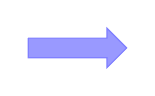
\begin{tikzpicture}
\path[draw=blue!50,fill=blue!40] (0,0.125) -- (1.0,0.125) -- (1.0,0.25) -- (1.25,0.0) -- (1.0,-0.25) -- (1.0,-0.125) -- (0.0,-0.125) -- (0.0,0.125);
\end{tikzpicture}
}

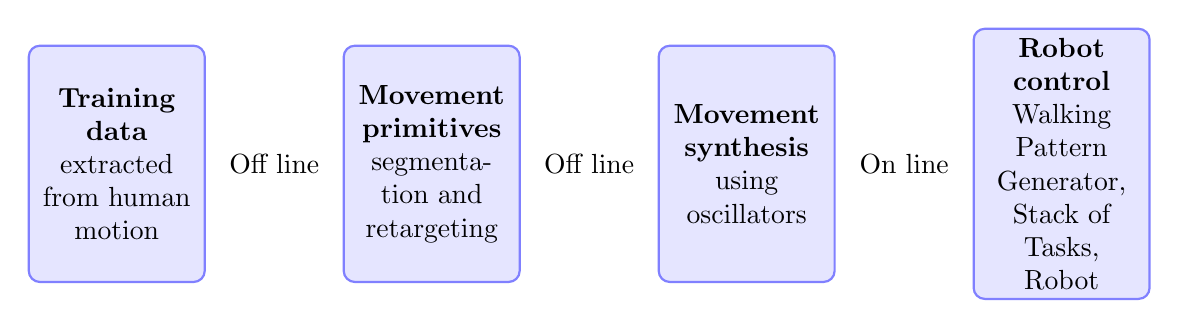
\begin{tikzpicture}%[show background grid]% every node/.style={draw,outer sep=0pt,thick}]

% Rectangle
\node (trainingdata) [text centered, shape=rectangle,rounded corners,draw=blue!50,fill=blue!10,thick,text width=2cm, minimum height=3cm]
  at (0.0,-0.5) {\textbf{Training data} extracted from human motion};

\node (movementprimitives) [text centered, shape=rectangle,rounded corners,draw=blue!50,fill=blue!10,thick,text width=2cm, minimum height=3cm]
  at (4.0,-0.5) {\textbf{Movement primitives} segmentation and retargeting};

\node (movementsynthesis) [text centered, shape=rectangle,rounded corners,draw=blue!50,fill=blue!10,thick,text width=2cm, minimum height=3cm]
  at (8.0,-0.5) {\textbf{Movement synthesis} using oscillators};

\node (robotcontrol) [text centered, shape=rectangle,rounded corners,draw=blue!50,fill=blue!10,thick,text width=2cm, minimum height=3cm]
  at (12.0,-0.5) {\textbf{Robot control}\\Walking Pattern Generator,\\ Stack of Tasks,\\ Robot};

\node (firstarrow) at (2.0,0.25) {\localarrow };

\node (sndarrow) at (6.0,0.25) {\localarrow };

\node (thrdarrow) at (10.,0.25) {\localarrow };

\node[rotate=180] (rfirstarrow) at (2.0,-1.25) {\localarrow };
\node[rotate=180] (rsndarrow) at (6.0,-1.25) {\localarrow };
\node[rotate=180] (rthrdarrow) at (10.,-1.25) {\localarrow };

\node (offline1) at ( 2.0,-0.5) {Off line};
\node (offline2) at ( 6.0,-0.5) {Off line};
\node (offline1) at (10.0,-0.5) {On line};

\end{tikzpicture}
}
  \end{center}
%  
\end{frame}

\begin{frame}{Implementation on HRP-2}
  %\vspace*{-0.8cm}  
  \begin{center}
    \scalebox{0.7}{%!TEX root = ../../14-icra-RealTimeNMPC.tex

\tikzstyle{block} = [draw=blue!50, fill=blue!20, rectangle,
    minimum height=2em, minimum width=5em, align=center]
\tikzstyle{point} = [coordinate]
\tikzstyle{pinstyle} = [pin edge={to-,thin,black}]

\definecolor{KPS}{RGB}{204 ,  85 , 0}% corail
\definecolor{SBG}{RGB}{222, 152, 22 }% melon
\definecolor{WPG}{RGB}{231 ,  62 , 1}% orange 
\definecolor{SOT}{RGB}{179, 103, 0}% cuivre
\definecolor{ROB}{RGB}{173, 79, 9} % roux
\definecolor{EST}{RGB}{255, 127, 0}

% The block diagram code is probably more verbose than necessary
\begin{tikzpicture}[auto, scale=1.0]
  \draw [fill=green,opacity=.1,text opacity=1] (2.2,1.0) rectangle (14,-2.2);
  \node at(11,-2.0) {\textcolor{green!20!black!100}{Stack of Task}};

    \node [block, text depth=0.7cm, minimum width=2.0cm] at (10.0,-3.0) (robot) {
        Robot
    };
    \node [block, text opacity=1, opacity=0, font=\small, minimum width=1.1cm ] at ([yshift=-0.2cm]robot.center){
      (position \\
      control)
    };
%%%%
    \node [block,  text depth=0.8cm, minimum width=3.0cm] at (5.0,-3.0) (estimator) {
      Estimator 
    };
    \node [block, text opacity=1, opacity=0, draw=white, font=\small, minimum width=1cm ] at ([yshift=-0.2cm]estimator.center){
      (robot and objects\\
      relative positions)
    };
%%%%
    \node [block,  minimum width=0.1cm] at (3.5,-1.0) (wpg) {
        Walking\\
        Pattern\\
        Generator
    };
%%%%
    \node [block,  minimum width=0.1cm, text depth = 0.18cm] at (7.0,-1.0) (dyn) {
        \\[0.1cm]
        Dynamic\\
        Filter
    };
%%%%%
    \node [block,  text depth = 0.7cm, minimum width=2.0cm] at (10.5,-0.5) (sot) {
      \\[0.1cm]
      Task for\\
      Trajectory\\
      Tracking
    };
%%    \node [block, text opacity=1, opacity=0, draw=white, font=\footnotesize, minimum width=1.5cm ] at ([yshift=-0.3cm]sot.center){
%%      (generalized\\
%%      inverse\\
%%      kinematics,\\
%%      SoT)
%    };
    \node [block,  text depth = 1.0cm, minimum width=1.0cm] at (13.1,-0.5) (qp){
      \\[0.5cm]      
      QP\\solver
    };
%%%%  
    \node [block,  minimum width=0.1cm] at (0.0, 0.0) (kps) {
    		Kinematic \\
      Pattern \\
      Synthesis
    	};
%%%%%%%%%%%%%%%%%%%%%%%%%%%%%%%%%%%%%%%%%%%%%%%%%%%%%%%%%%%%%%%%%%%%%%%%%%%%%%%%%%%%%%%%%%
    % PATHS
    	% Forward chaine
    	\node [point] at ([xshift=-0.5cm]wpg.west) (walkingwest) {};
    \draw [ - ] ([yshift=-0.3cm]kps) -| node {} (walkingwest);
    \draw [ ->] (walkingwest) |- node [left] {\small $[{\mathbf v}^{\,{\text{ref}}}\;,\;{\mathbf \omega}^{\,{\text{ref}}}]$} (wpg.west);
%%%%    
    	\node [point] at ( $(dyn.west) + (-0.4,1.0)$ ) (dynwest) {};
    \draw [ - ] ([yshift=+0.1cm]kps) -- node  [above] {\small ${\mathbf q}^{\,{\text{upper body}}}$} (dynwest);
    \draw [ ->] (dynwest) |- node {} ([yshift=+0.3cm]dyn.west);    
    \draw [ ->] (dynwest) |- node {} ([yshift=+0.5cm]sot.west);
%%%%
    \draw [->] ([yshift=-0.1cm]wpg.east) -- node [below , font=\small] {} ([yshift=-0.1cm]dyn.west);
    \node [block, text opacity=1, opacity=0, font=\scriptsize, minimum width=0.01cm] at ($(dyn.west) + (-0.9,-0.7)$){
      CoM$^{ref,{\bf 1}}$ \\ ZMP$^{ref}$ \\ Feet$^{ref}$
    };
%%%%
    \draw [->] (dyn.east) -- node {} ([yshift=-0.5cm]sot.west);
    \node [block, text opacity=1, opacity=0, font=\scriptsize, minimum width=0.01cm] at ($(sot.west) + (-0.9,-1.1)$){
      CoM$^{ref,{\bf 2}}$ \\ ZMP$^{ref}$ \\ Feet$^{ref}$
    };
    
    \draw [draw,->] (sot) -- node {\small Tasks} (qp.west);

   	% Feedback chaine
    	\node [point] at ($(sot.east) + (0.1,0.0)$) (soteast) {};
    \draw [draw,->] (qp) |- node {\small ${\mathbf q},\dot{{\mathbf q}},\ddot{{\mathbf q}}$} (robot);
    
    \draw [draw,->] (robot) -- node {\small sensors data} (estimator);
    
    \draw [draw,->] (estimator) -| node [below right = 0.0cm and 0.5cm]{\small scene parameters} ($(kps.south)+ (-0.1,0.0)$);

    
%%%%%%%%%%%%%%%%%%%%%%%%%%%%%%%%%%%%%%%%%%%%%%%%%%%%%%%%%%%%%%%%%%%%%%%%%%%%%%%%%%%%%%%%5
\end{tikzpicture}

}
  \end{center}
%  
  \begin{itemize}
    \item The upper body is learned from humans.
    \item The lower body is computed via NMPC.
    \item The Dynamic Filter links them.
  \end{itemize}
\end{frame}

\begin{frame}{Motion on HRP-2}
  \begin{center}
    \movie[autostart,loop]{
    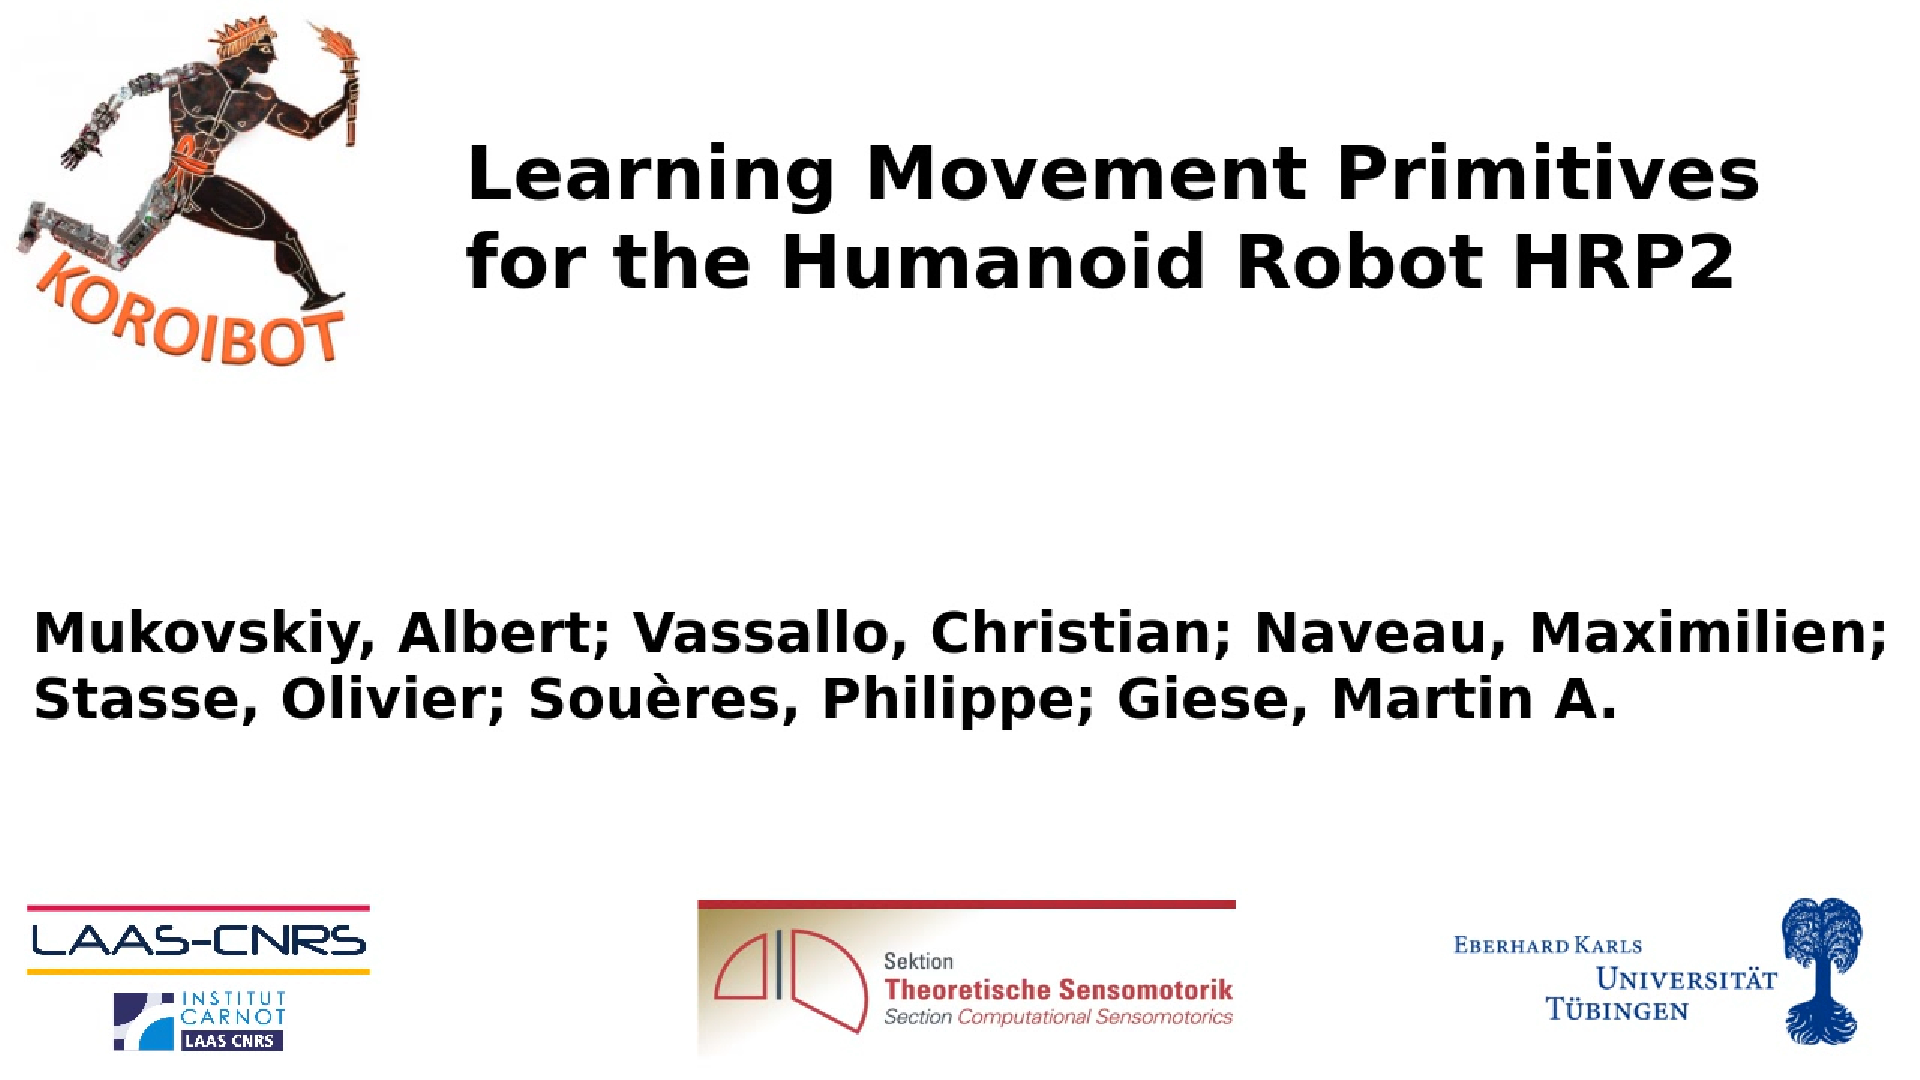
\includegraphics[width=0.9\linewidth, keepaspectratio]
      {motion_primitives/16-mukovskiy-elsarticle.png}    
    }  
    {./videos/16-mukovskiy-elsarticle.mp4}
  \end{center}
\end{frame}


